%%%%%%%%%%%%%%%%%%%%%%%%%%%%%%%%%%%%%%%%%%%%%%%%%%%%%%%%%%%%%%%%%%%
%                                                                 %
%                            APPENDICES                           %
%                                                                 %
%%%%%%%%%%%%%%%%%%%%%%%%%%%%%%%%%%%%%%%%%%%%%%%%%%%%%%%%%%%%%%%%%%%
 
\appendix    % This command is used only once!
%\addcontentsline{toc}{chapter}{APPENDICES}             %toc entry  or:
\addtocontents{toc}{\parindent0pt\vskip12pt APPENDICES} %toc entry, no page #

\chapter{Ontologies}
\section{PROV-PUB-O/S serialized in Turtle (TTL)}
\lstinputlisting{model/prov-pub-s4listing.ttl}
\section{PROV-PUB-O/S to DoCO bridging ontology}
\lstinputlisting{model/prov-pub-s-doco4listing.ttl}
\section{PROV-PUB-O/S to BIBO bridging ontology}
\lstinputlisting{model/prov-pub-s-bibo4listing.ttl}
\section{PROV-PUB-O/S to BibTeX bridging ontology}
\lstinputlisting{model/prov-pub-s-bibtex4listing.ttl}
\section{PROV-PUB-O/S usage examples}
\lstinputlisting{model/prov-pub-s-examples4listing.ttl}

\chapter{Case study details of the 5 figures and 3 tables in Chapter 4 of NCA 2014 report}
The case study is performed on Chapter 4, ``Energy supply and use'' of the National Climate Assessment Report 2014.

Chapter URI is \url{http://data.globalchange.gov/report/nca3/chapter/energy-supply-and-use}
Turtle file is \url{http://data.globalchange.gov/report/nca3/chapter/energy-supply-and-use.ttl}
This URL pattern applies for all the URIs below.

Figure 4.1 is ``Paths of Hurricanes Katrina and Rita Relative to Oil and Gas Production Facilities''. The
figure URI is \url{http://data.globalchange.gov/report/nca3/chapter/energy-supply-and-use/figure/paths-of-hurricanes-katrina-and-rita-relative-to-oil-and-gas-production-facilities}.
This figure was derived from \url{http://data.globalchange.gov/report/gao-06-420t} --- ``Natural Gas: Factors Affecting Prices and Potential Impacts on Consumers (GAO-06-420T)'', the 
PDF file of this ``GAO-06-420T'' report is available at \url{http://www.gao.gov/assets/120/112796.pdf}.
Actually Figure 4.1 of NCA 2014 is almost the same as Figure 3 of the ``GAO-06-420T'' report, which has a note reads ``Source: GAO analysis of data provided by the National Weather Service and the Minerals Management Service.''
Only legends are found changed.

Figure 4.2 is ``Increase in Cooling Demand and Decrease in Heating Demand''. The
percent differences are compared to the average for 1970-2000
Figure URI is \url{http://data.globalchange.gov/report/nca3/chapter/energy-supply-and-use/figure/increase-in-cooling-demand-and-decrease-in-heating-demand}
This figure was derived from \url{http://data.globalchange.gov/report/aeo2008} --- ``Annual Energy Outlook 2008 With Projections to 2030'', available at \url{http://www.eia.gov/oiaf/aeo/pdf/0383(2008).pdf}, but no clue relevant to this figure is found in this report.
The figure has an image \url{http://data.globalchange.gov/image/e7bdf318-1e1f-4c85-821f-907a55ff0ede}, which was derived from \url{http://data.globalchange.gov/dataset/nca3-heating-cooling-degree-day-data-r1}, which has a landing page at \url{http://www.ncdc.noaa.gov/oa/documentlibrary/hcs/hcs.html}. Footnote 16 of the chapter in NCA 2014 also says that data come from \url{http://www.ncdc.noaa.gov/oa/documentlibrary/hcs/hcs.html}
Raw data could be obtained by filling out the form at \url{http://www7.ncdc.noaa.gov/CDO/CDODivisionalSelect.jsp#} put for period 1970.1---2010.12.
This service is found by following a link at the hcs.html page: ``Item 14 on the NCDC Quick Links page'', and then click the ``Climate Indices'' hyperlink.
Temporary link to the raw data file was \url{http://www1.ncdc.noaa.gov/pub/orders/CDODiv8103636830652.txt}
Space separated raw data file can be found at  \url{http://www1.ncdc.noaa.gov/pub/orders/CDODiv2177686828992.txt}
This file became inaccessible after some time, so if we want to download the data again, we need to resubmit the request instead of re-accessing the temporary link to the raw data file.
A Jupyter Notebook --- nca3chapter4figure2no-output.ipynb --- was created which almost reproduced the result figure --- Figure 4.2.
Code of the Jupyter Notebook is shown in Figure~\ref{fig:nca3code} and the reproduced figure is shown in Figure~\ref{fig:nca3image}.
\begin{figure}
	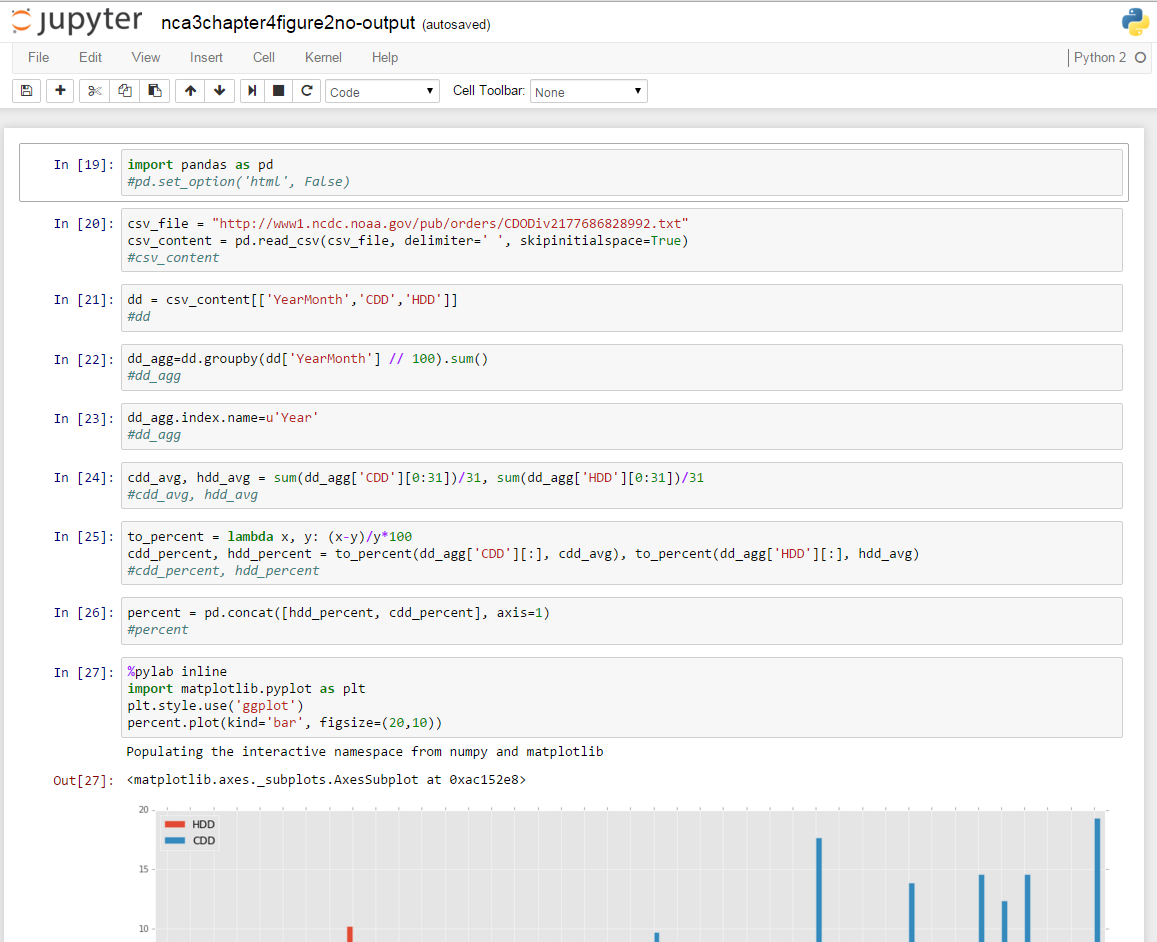
\includegraphics[width=\textwidth]{nca3code.png}
	\caption{Code reproducing Figure 4.2 of NCA 2014}
	\label{fig:nca3code}
\end{figure}
\begin{figure}
	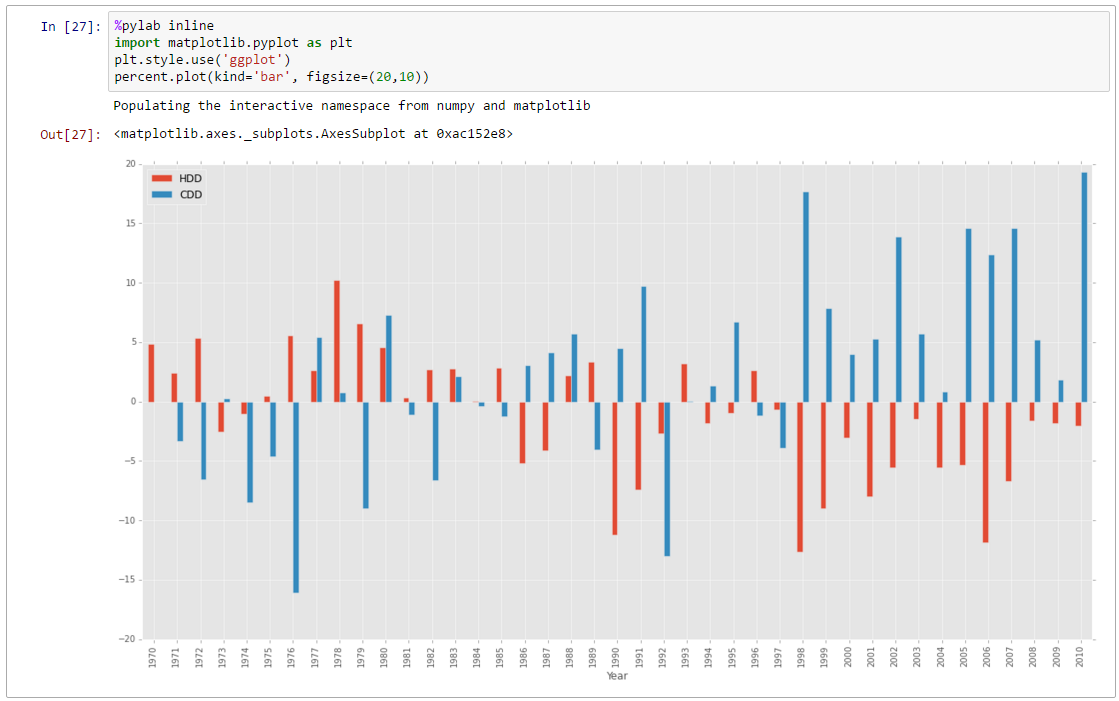
\includegraphics[width=\textwidth]{nca3image.png}
	\caption{The reproduced figure similar to Figure 4.2 of NCA 2014}
	\label{fig:nca3image}
\end{figure}

The textual description given in the caption of the figure is as follows:
\begin{quotation}
The amount of energy needed to cool (or warm) buildings is proportional to cooling (or heating) degree days. The figure shows increases in population-weighted cooling degree days, which result in increased air conditioning use, and decreases in population-weighted heating degree days, meaning less energy required to heat buildings in winter, compared to the average for 1970-2000. Cooling degree days are defined as the number of degrees that a day's average temperature is above 65°F, while heating degree days are the number of degrees a day’s average temperature is below 65°F. As shown, the increase in cooling needs is greater than the decrease in heating needs (Data from NOAA NCDC 2012).

\end{quotation}

%!wget --output-document=input.txt http://www1.ncdc.noaa.gov/pub/orders/CDODiv169846853945.txt -- physical change
%csv_content_1 = pd.read_csv("input.txt", delimiter=' ', skipinitialspace=True) -- syntactical change
%dd = csv_content_1[['YearMonth','CDD','HDD']] -- semantical change
%the e7bdf318-nca3-heating-cooling-degree-day-data-r1-process generated this image, but does not include a “qualifiedAssociation/hadPlan” field to describe the detailed process of image generation.
%describe the relationship among percent and img and figure 4.2 -- plot (syntactical change) and then reuse (concerning result, not data) result = display of data 
%figure 4.3 Increasing Numbers of Cooling Degree Days
%figure uri: http://data.globalchange.gov/report/nca3/chapter/energy-supply-and-use/figure/cooling-degree-days
%this figure cites the article titled "U.S. Population Projections", accessible at http://www.census.gov/population/projections/, the article is not directly related to the figure, but just an additional comment to the figure (population projections suggest continued shifts toward areas that require air conditioning in the summer).
%This figure mentioned in its caption that the figure source is NOAA NCDC / CICS-NC, but cannot find the related resources by searching with these keywords on the Web.
%A2 and B1 are two scenarios defined in the IPCC (Intergovernmental Panel on Climate Change) Special Report on Emission Scenarios (SRES)
%its four images such as http://data.globalchange.gov/image/f6db3545-873b-4c9e-b857-c3bb5671aea4, “Increasing Numbers of Cooling Degree Days: Higher Emissions (A2), 2021-2050”, are all derived from the dataset "nca3-cmip3-downscaled-r201304". the dataset has a landing page http://cida.usgs.gov/thredds/catalog.html. its title is "Eighth degree-CONUS Daily Downscaled Climate Projections", a report on this dataset can be found at http://cida.usgs.gov/thredds/fileServer/dcp/files/Hayhoe_USGS_downscaled_database_final_report.pdf. but the report is not helpful to finding the provenance.
%following a link at http://cida.usgs.gov/thredds/catalog.html, at http://cida.usgs.gov/thredds/catalog.html?dataset=cida.usgs.gov/thredds/dcp/conus_t, a dataset called "1/8 degree-CONUS Daily Downscaled Climate Projections Minimum and Maximum Temperature" is found. It has a lot of variables together: ccsm, cgcm3-t47, cgcm3-t63, cnrm, csiro, echam5, echo, gfdl, giss_aom, hadcm3, hadgem, miroc_hi, mri_cgcm2, pcm. 
%we can use the netCDF subset service at http://cida.usgs.gov/thredds/ncss/dcp/conus_t/dataset.html to download a subset of the dataset as a netCDF file. One year of ccsm a2 tmax data are 286MB in size.
%NCSS Request URL is of the form http://cida.usgs.gov/thredds/ncss/dcp/conus_t?var=ccsm-a2-tmax-NAm-grid&disableLLSubset=on&disableProjSubset=on&horizStride=1&time_start=1960-01-01T00%3A00%3A00Z&time_end=2099-12-31T00%3A00%3A00Z&timeStride=1
%!wget 
%http://cida.usgs.gov/thredds/uddc/dcp/conus_t?catalog=http%3A%2F%2Fcida.usgs.gov%2Fthredds%2Fcatalog.html&dataset=cida.usgs.gov%2Fthredds%2Fdcp%2Fconus_t has title: Eighth degree-CONUS Daily Downscaled Climate Projections by Katharine Hayhoe, exact match with the dataset description in the data.globalchange.gov!!! but it is just a quality assessment of the data set in terms of attribute convention.
%prov:hadPlan field of the prov:qualifiedAssociation field of the process “http://data.globalchange.gov/activity/f6db3545-nca3-cmip3-downscaled-r201304-process” describes the algorithm:
%1. For each model at each grid point, the number of cooling degree days under the higher emissions scenario (A2) was calculated for two periods: 1971-2000 and 2021-2050. According to the figure 4.2 caption, “Cooling degree days are defined as the number of degrees that a day’s average temperature is above 65ºF”, yet the dataset has no “average temperature” variable, but only max and min temperature values. How is the number of cooling degree days calculated is unclear.
%2. At each grid point, the number of cooling degree days was computed for both time periods by averaging the following models:
%- cgcm3_t47
%- cgcm3_t63
%- cnrm
%- echam5
%- echo
%- gfdl_2.1
%- hadcm3
%- pcm
%3. At each grid point, the difference in the number of cooling degree days was calculated for 2021-2050 minus 1971-2000.
%4. Data were plotted for all grid points.
%image http://data.globalchange.gov/image/f6db3545-873b-4c9e-b857-c3bb5671aea4, “Increasing Numbers of Cooling Degree Days: Higher Emissions (A2), 2021-2050”, was generated by the above process.
%
%figure 4.4 Projected Changes in Seasonal Precipitation
%figure uri: http://data.globalchange.gov/report/nca3/chapter/energy-supply-and-use/figure/projected-changes-in-seasonal-precipitation
%the same as 4.3, this figure also cites NOAA NCDC / CICS-NC
%its upper-left image --- "Projected Changes in Seasonal Precipitation - Winter" (uri: http://data.globalchange.gov/image/5ae3d8d8-64d1-4dab-a08a-4ec46a58e3da) --- was derived from World Climate Research Programme's (WCRP's) Coupled Model Intercomparison Project phase 3 (CMIP3) multi-model dataset, the identifier of the dataset is dataset/nca3-cmip3-r201205, and the landing page is http://www-pcmdi.llnl.gov/ipcc/about_ipcc.php, downloading the data requires registration and approval from the administrator. It took 4 days to finish my registration process.
%"/activity/5ae3d8d8-nca3-cmip3-r201205-process" has description of the activity generating the image.
%(All the four images in this figure are described in the same manner.)
%the plan (prov:qualifiedAssociation/prov:hadPlan) for the process (hopefully how to use the data at http://www-pcmdi.llnl.gov/ipcc/about_ipcc.php): 
%1. For each model at each grid point, the mean winter precipitation under the higher emissions scenario (A2) was calculated.
%2. For each model, these data were re-gridded to a common grid.
%3. For each model at each grid point, the mean winter precipitation under the higher emissions scenario (A2) was calculated for two periods: 1970-1999 and 2041-2070.
%4. At each grid point, the mean winter precipitation for the two periods was computed by averaging the following models: how “mean winter precipitation” is calculated is unclear. because only daily, weekly, monthly and yearly means are given in the data files for the following models. BTW, the portal is having issues with data browsing and downloading.
%CCSM3, CGCM3.1 (T47), CNRM-CM3, CSIRO-Mk3.0, ECHAM5/MPI-OM, ECHO-G, GFDL-CM2.0, GFDL-CM2.1, INM-CM3.0, IPSL-CM4, MIROC3.2 (medres), MRI-CGCM2.3.2, PCM, UKMO-HadCM3, and UKMO-HadGEM1
%5. At each grid point, the difference in projected winter precipitation was calculated for 2041-2070 minus 1970-1999.
%6. Data were plotted for grid points in the United States with hatching/white-out applied as follows:
%If less than 50% of the models show a statistically significant change, then those grid points are whited out. If more than 50% of the models show a statistically significant change, but less than 67% of the models agree on the sign of the change, then those grid points are shaded. If more than 50% of the models show a statistically significant change, and more than 67% of the models agree on the sign of the change, then shading is overlaid with hatching for those grid points. 
%following a link at http://www-pcmdi.llnl.gov/ipcc/about_ipcc.php, we get to the page http://www-pcmdi.llnl.gov/ipcc/orientation.php, which has a link to http://www-pcmdi.llnl.gov/ipcc/data_status_tables.htm, we can see SRESA2 is among the column titles, and CCSM3, CGCM3.1 (T47), CNRM-CM3, CSIRO-Mk3.0, ECHAM5/MPI-OM, ECHO-G, GFDL-CM2.0, GFDL-CM2.1, INM-CM3.0, IPSL-CM4, MIROC3.2 (medres), MRI-CGCM2.3.2, PCM, UKMO-HadCM3, and UKMO-HadGEM1, others in the table are not included by the process.
%following another link at http://www-pcmdi.llnl.gov/ipcc/about_ipcc.php, we get to https://esg.llnl.gov:8443/about/ipccTables.do, where we know that “pr” is for Precipitation.
%yet another link at http://www-pcmdi.llnl.gov/ipcc/about_ipcc.php  to https://esg.llnl.gov:8443/about/search.do instructs users how to search the datasets.
%at https://esg.llnl.gov:8443/data/advancedSearchPage.do, we can search for SRES A2 experiment, CGCM3.1 T47 and get Run1--5 monthly data
%The site is having issues with data browsing and downloading, we are advised to go to ftp://ftp-esg.ucllnl.org instead, where we can find a sresa2 directory, with 4 empty files… there is a ftp sitemap at https://esg.llnl.gov:8443/about/ftp.do, which points us to sresa2, the empty directory…
%
%figure 4.5 California Power Plants Potentially at Risk from Sea Level Rise
%uri: http://data.globalchange.gov/report/nca3/chapter/energy-supply-and-use/figure/california-power-plants-potentially-at-risk-from-sea-level-rise
%is derived from "Estimating Risk to California Energy Infrastructure from Projected Climate Change", 
%uri: http://data.globalchange.gov/report/osti-1026811 
%found at http://www.energy.ca.gov/2012publications/CEC-500-2012-057/CEC-500-2012-057.pdf, but no direct link to this paper source.
%Figure 19. Power Plants Potentially at Risk to a 100-year Flood with a 1.4 m Sea Level Rise, not specified and this is a 88-page report.
%
%table 4.1 Changing Energy Use for Heating and Cooling Will Vary by Region
%uri: http://data.globalchange.gov/report/nca3/chapter/energy-supply-and-use/table/energy-regional-impacts
%the table cites "noaa-techreport-nesdis-142-[1-6]" each of these citations’ gcis:hasURL points to the pdf file of the report.
%table caption says “Table information is adapted from multi-model means from 8 NARCCAP regional climate simulations for the higher emissions scenario (A2) considered in this report and is weighted by population.” in reference 20, the 6 reports this table is based on are listed.
%how these days are weighted by population? what kind of adaptation has been done? is the adaptation just the “population weighting” calculation?
%142-1: northeast, figure 25 and 26 is about 2041-2070 mean minus 1980-2000 mean.
%table 5’s in 142-[1-6] have relevant data but different values.
%table 4.1 says for northeast +10 days extreme hot days (>95F), but table 5 of 142-1 says +8 days for NARCCAP Mean and +4 days for Daily_CMIP3 Mean, and table 4.1 says +77% increase in CDDs per year (2041-2070 above 1971-2000), but table 5 says +99% for NARCCAP Mean and +91% for Daily_CMIP3 Mean.
%Northeast:
%Source	Additional >95F days	% increase in CDDs	Fewer <10F days	% decrease in HDDs
%Table 4.1 in NCA3	+10 days	+77%	-12 days	-17%
%Table 5 in 142-1, NARCCAP Mean	+8 days	+99%	-17 days	-16%
%Daily_CMIP3 Mean	+4 days	+91%	-13 days	-18%
%Southeast:
%Source	Additional >95F days	% increase in CDDs	Fewer <10F days	% decrease in HDDs
%Table 4.1 in NCA3	+23 days	+43%	-2 days	-19%
%NARCCAP Mean	+27 days	+49%	-2 days	-19%
%Daily_CMIP3 Mean	+33 days	+42%	-1 days	-23%
%Midwest:
%Source	Additional >95F days	% increase in CDDs	Fewer <10F days	% decrease in HDDs
%Table 4.1 in NCA3	+14 days	+64%	-14 days	-15%
%NARCCAP Mean	+15 days	+66%	-16 days	-16%
%Daily_CMIP3 Mean	+13 days	+75%	-13 days	-17%
%Great Plains:
%Source	Additional >95F days	% increase in CDDs	Fewer <10F days	% decrease in HDDs
%Table 4.1 in NCA3	+22 days	+37%	-4 days	-18%
%NARCCAP Mean	+18 days	+48%	-12 days	-16%
%Daily_CMIP3 Mean	+25 days	+53%	-10 days	-17%
%Southwest:
%Source	Additional >95F days	% increase in CDDs	Fewer <10F days	% decrease in HDDs
%Table 4.1 in NCA3	+20 days	+44%	-3 days	-20%
%NARCCAP Mean	+20 days	+64%	-11 days	-18%
%Daily_CMIP3 Mean	+24 days	+65%	-8 days	-19%
%Northwest:
%Source	Additional >95F days	% increase in CDDs	Fewer <10F days	% decrease in HDDs
%Table 4.1 in NCA3	+5 days	+89%	-7 days	-15%
%NARCCAP Mean	+5 days	+105%	-15 days	-15%
%Daily_CMIP3 Mean	+10 days	+147%	-9 days	-16%
%
%table 4.2 Possible Climate Resilience and Adaptation Actions in Energy Sector
%uri: http://data.globalchange.gov/report/nca3/chapter/energy-supply-and-use/table/energy-adaptation
%the table cites http://data.globalchange.gov/report/ornl-climchinfrastructure-2012, which has URL http://www.esd.ornl.gov/eess/Infrastructure.pdf
%it is a table listing items and their attributes, instead of the result of changes of data.
%table 4.3 Energy Supply: Summary of National and Regional Impacts, Challenges and Opportunities
%uri: http://data.globalchange.gov/report/nca3/chapter/energy-supply-and-use/table/energy-supply-national-regional
%this table cites http://data.globalchange.gov/report/ornl-climchinfrastructure-2012, and http://data.globalchange.gov/report/ccsp-sap-2_1a-2007, which has URL http://downloads.globalchange.gov/sap/sap2-1a/sap2-1a-final-all.pdf
%notes for column “mean annual temperature” and “summer precipitation”: CMIP3 15 GCM Models: 2070–2099 Combined Interquartile Ranges of SRES B1 and A2 (versus 1971–2000), incorporating uncertainties from both differences in model climate sensitivity and differences between B1 and A2 in emissions trajectories 
%notes for “sea level rise (2100)”: Range of sea level rise for 2100 is the Low Intermediate to High Intermediate Scenario from “Sea Level Change Scenarios for the U.S. National Climate Assessment.”35 Range is similar to the 1 to 4 feet of sea level rise projected in Ch. 2: Our Changing Climate, Key Message 10. There will be regional variations in sea level rise, and this category of impacts does not apply for the Midwest region.
%notes for “#Days >90F (2055)” has references http://data.globalchange.gov/report/ornl-climchinfrastructure-2012 and http://data.globalchange.gov/report/ccsp-sap-2_1a-2007, how these numbers are obtained not found yet.


%This is how equations are numbered in an appendix:
%\begin{equation}
%x^2 + y^2 = z^2
%\end{equation} 
%This is a sentence to take up space and look like text.
%This is a sentence to take up space and look like text.
%This is a sentence to take up space and look like text.
% 
%This is a sentence to take up space and look like text.
%This is a sentence to take up space and look like text.
%This is a sentence to take up space and look like text.
%This is a sentence to take up space and look like text.
%This is a sentence to take up space and look like text. 

%\chapter{THIS IS ANOTHER APPENDIX} 
%This is a sentence to take up space and look like text.
%This is a sentence to take up space and look like text.
%This is a sentence to take up space and look like text.
%This is a sentence to take up space and look like text.
%This is a sentence to take up space and look like text.
%This is a sentence to take up space and look like text.
%This is a sentence to take up space and look like text.
%This is a sentence to take up space and look like text.
 
